\documentclass[12pt,a4paper]{article}

% Paquetes básicos
\usepackage[utf8]{inputenc}
\usepackage[T1]{fontenc}
\usepackage[spanish, es-tabla]{babel}
\addto\captionsspanish{\renewcommand{\tablename}{Táboa}}
\addto\captionsspanish{\renewcommand{\listtablename}{Índice de táboas}}
\usepackage{graphicx}
\usepackage{amsmath}
\usepackage{amssymb}
\usepackage{hyperref}
\usepackage{geometry}
\usepackage{listings}
\usepackage{xcolor}
\usepackage{float}
\usepackage{epigraph}
\usepackage{cite}
\usepackage[listings]{tcolorbox}
\tcbuselibrary{listings, skins, breakable}
\lstloadlanguages{SQL}
\usepackage{subcaption}
\usepackage{url}
\usepackage{booktabs}
\usepackage{tabularx}
\usepackage{array}
\usepackage{enumitem}
\usepackage{setspace}
\usepackage{tikz}
\usetikzlibrary{arrows.meta, positioning, shapes.geometric}

% Configurar márgenes
\geometry{
    top=2cm,
    bottom=2cm,
    left=2cm,
    right=2cm
}

\setstretch{1.08}
\setlength{\parindent}{0pt}
\setlength{\parskip}{0.45em}
\renewcommand{\arraystretch}{1.18}

% Configurar listings
\lstset{
    extendedchars=true,
    inputencoding=utf8,
    basicstyle=\small\ttfamily,
    breaklines=true,
    frame=single,
    numbers=left,
    numberstyle=\tiny,
    captionpos=b
}

% Información del documento
\title{Adestramento de modelos de IA}
\author{Laura Cabaleiro Pintos \& Pablo Chantada Saborido \\ Marcelo Ferreiro Sánchez \& José Romero Conde}
\date{Curso 2025--2026}

\lstdefinelanguage{SQL}{
  morekeywords={
    SELECT,FROM,WHERE,AND,OR,INSERT,INTO,VALUES,UPDATE,SET,DELETE,CREATE,TABLE,
    ALTER,DROP,JOIN,INNER,LEFT,RIGHT,FULL,ON,AS,ORDER,BY,GROUP,HAVING,DESC,ASC,
    DISTINCT,COUNT,SUM,AVG,MIN,MAX,IN,IS,NOT,NULL,LIKE,BETWEEN,EXISTS,UNION
  },
  sensitive=false,
  morecomment=[l]{--},
  morecomment=[s]{/*}{*/},
  morestring=[b]',
  morestring=[b]"
}

\definecolor{azulito}{RGB}{186,200,211}
\definecolor{azul_oscuro}{RGB}{35,68,93}
\definecolor{turquesa}{RGB}{174,143,171}
\definecolor{terminalbg}{RGB}{255,255,255}

\lstset{
  language=SQL,
  basicstyle=\color{azul_oscuro}\ttfamily\small,
  keywordstyle=\color{white}\bfseries,
  commentstyle=\color{gray}\itshape,
  stringstyle=\color{turquesa},
  backgroundcolor=\color{azulito},
  frame=single,
  numbers=left,
  numberstyle=\tiny\color{gray},
  breaklines=true,
  tabsize=2
}

\lstdefinestyle{terminal}{
    backgroundcolor=\color{terminalbg},
    basicstyle=\ttfamily\small\color{azul_oscuro},
    frame=single,
    breaklines=true,
    showstringspaces=false,
}

\hypersetup{
    colorlinks=true,
    linkcolor=black,
    urlcolor=blue,
    citecolor=black,
    pdftitle={Adestramento de modelos de IA},
    pdfauthor={Marcelo Ferreiro Sánchez, Pablo Chantada Saborido, Laura Cabaleiro Pintos, Pepe Romero Conde}
}

\begin{document}

\maketitle

\tableofcontents

\newpage

\section{Introdución}

Neste traballo empréganse dous modelos de intelixencia artificial sobre o
dataset CIC-IDS2017 co obxectivo de estudar a súa aplicación nun sistema de
detección de intrusións a nivel de rede. Os modelos escollidos foron
AdaBoost \cite{freund1996experiments} como modelo base e
GAN \cite{goodfellow2014generative} como modelo complexo.

O obxectivo principal da práctica é resolver un problema de clasificación
binaria, no que cada fluxo debe etiquetarse como \texttt{BENIGN} ou
\texttt{ATTACK}. Ademais, como extensión, tamén se analiza o comportamento
de AdaBoost no escenario multiclase, empregando as etiquetas orixinais do
dataset.

Nesta segunda parte da práctica non se realiza de novo o preprocesado
completo, senón que se parte do conxunto de datos xa preparado na entrega
anterior. O traballo céntrase, por tanto, no adestramento, avaliación e
comparación dos modelos, así como na análise das dificultades atopadas e das
prestacións acadadas en cada caso.

\section{Dataset empregado}

O dataset empregado neste traballo procede do preprocesado realizado na primeira práctica. 
Partiuse da versión completa \texttt{TrafficLabelling} de CIC-IDS2017, sobre a que se eliminaron filas baleiras, valores nulos, valores infinitos, 
columnas duplicadas ou sen información útil e variables con alto risco de introducir sesgo, como identificadores de fluxo, IPs e marcas temporais.

Tras a limpeza inicial, o conxunto útil quedou en 2\,827\,876 fluxos. As variables categóricas principais, como portos e protocolo, foron codificadas 
numericamente, agrupando portos pouco frecuentes nunha categoría común. As variables numéricas foron normalizadas e posteriormente realizouse unha 
selección de características apoiada en PCA, mantendo finalmente 52 características predictoras.

Debido ao forte desbalanceo entre clases, aplicouse unha combinación de \emph{undersampling} nas clases maioritarias e SMOTE nas clases minoritarias. 
O dataset final usado nesta práctica quedou composto por 182\,000 mostras. A partición realizouse de forma estratificada cun reparto 70/15/15, obtendo 
127\,400 mostras de adestramento, 27\,300 de validación e 27\,300 de test.

No escenario binario, a etiqueta \texttt{BENIGN} codificouse como clase negativa e todas as demais etiquetas como clase positiva \texttt{ATTACK}. 
Esta mesma partición foi empregada tanto para AdaBoost como para a GAN.


\section{GAN}

\subsection{Motivación e formulación}

A GAN empregouse como modelo complexo da práctica. Durante o desenvolvemento
probáronse varias formulacións.

Nun primeiro intento, a GAN formulouse como un detector de anomalías. Para iso,
o discriminador adestrábase só con exemplos \texttt{BENIGN} do conxunto de
adestramento balanceado e con mostras sintéticas xeradas a partir de ruído.
A idea era que o discriminador aprendese a recoñecer tráfico benigno e que,
na avaliación, os fluxos cun score baixo fosen considerados anomalías ou
ataques.

Despois probouse unha segunda variante do mesmo enfoque, empregando un
conxunto máis amplo de exemplos benignos extraídos do dataset orixinal.
Esta segunda proba foi tamén exploratoria e serviu para comparar o
comportamento da GAN cando se lle fornecían só mostras benignas do conxunto
balanceado fronte ao caso no que se empregaban moitos máis exemplos benignos
procedentes do conxunto inicial.

A versión final implementada foi distinta. O discriminador recibe mostras reais
do conxunto de adestramento e optimízase coa súa etiqueta binaria:
\texttt{BENIGN} como clase negativa e \texttt{ATTACK} como clase positiva.
Ademais, tamén recibe mostras sintéticas xeradas pola GAN, que se empregan
como exemplos artificiais coa etiqueta 0 durante o adestramento do
discriminador. Pola súa banda, o xerador optimízase para producir mostras que
o discriminador clasifique como 1.

Polo tanto, a versión final non é unha GAN non supervisada clásica nin unha
GAN condicionada. É unha formulación adversaria híbrida: o discriminador
aproveita as etiquetas binarias reais como obxectivo da perda, pero a etiqueta
non se introduce como entrada da rede.

\subsection{Arquitectura implementada}

A arquitectura final é deliberadamente sinxela. O xerador recibe un vector latente de tamaño \texttt{z\_dim} e produce unha mostra sintética co mesmo 
número de características ca o dataset. O discriminador recibe unha mostra do espazo de entrada e devolve un único logit para a clasificación binaria.

\begin{figure}[H]
\centering
\resizebox{0.98\textwidth}{!}{
\begin{tikzpicture}[
    box/.style={
        rectangle,
        rounded corners,
        draw=black,
        thick,
        align=center,
        minimum width=3.0cm,
        minimum height=1.15cm,
        fill=azulito!35
    },
    trainbox/.style={
        rectangle,
        rounded corners,
        draw=black,
        thick,
        align=center,
        minimum width=4.0cm,
        minimum height=1.05cm,
        fill=turquesa!20
    },
    arrow/.style={-{Latex[length=3mm]}, thick}
]

% ---------------- Xerador ----------------
\node[box] (z) {$z$\\\small Espazo latente};
\node[box, right=1.45cm of z] (g1) {128\\\small ReLU};
\node[box, right=1.45cm of g1] (g2) {256\\\small ReLU};
\node[box, right=1.45cm of g2] (gx) {$x_{dim}$\\\small Mostra sintética};

\draw[arrow] (z) -- (g1);
\draw[arrow] (g1) -- (g2);
\draw[arrow] (g2) -- (gx);

\node[above=0.45cm of g2] {\Large\textbf{Xerador}};

% ---------------- Discriminador ----------------
\node[box, below=2.25cm of z] (x) {$x_{dim}$\\\small Mostra de entrada};
\node[box, right=1.20cm of x] (d1) {256\\\small ReLU};
\node[box, right=1.20cm of d1] (drop) {Dropout};
\node[box, right=1.20cm of drop] (d2) {128\\\small ReLU};
\node[box, right=1.20cm of d2] (y) {1\\\small Logit};

\draw[arrow] (x) -- (d1);
\draw[arrow] (d1) -- (drop);
\draw[arrow] (drop) -- (d2);
\draw[arrow] (d2) -- (y);

\node[above=0.45cm of drop] {\Large\textbf{Discriminador}};

% ---------------- Adestramento ----------------
\node[trainbox, below=1.55cm of drop, xshift=-2.3cm] (loss) {\texttt{BCEWithLogitsLoss}};
\node[trainbox, right=1.3cm of loss] (adam) {Adam\\\small $lr=10^{-4}$, $\beta_1=0{,}5$, $\beta_2=0{,}999$};

\node[above=0.18cm of loss, xshift=2.65cm] {\textbf{Adestramento}};

\end{tikzpicture}
}
\caption{Arquitectura da GAN empregada. O xerador transforma un vector latente nunha mostra sintética co mesmo número de características ca entrada, mentres que o discriminador devolve un único logit para a clasificación binaria.}
\end{figure}

Tamén se parametrizaron o \emph{dropout}, o tamaño do lote, a frecuencia de avaliación e a dimensión do espazo latente. Isto permitiu facer probas curtas para verificar o funcionamento da tubaxe e probas longas para intentar estabilizar o adestramento.

\subsection{Resultados da clasificación binaria co discriminador}

As primeiras execucións conservadas da GAN foron probas curtas de só 6 épocas,
realizadas para comprobar que a tubaxe funcionaba correctamente. Nesas probas
o modelo aínda non converxía: a AUC-ROC de validación quedaba arredor de
0,74--0,78 e a accuracy arredor de 0,45--0,47. Estes valores indican que o
adestramento adversario necesitaba moitas máis épocas para estabilizarse.

Posteriormente realizouse un adestramento máis longo, con métricas rexistradas
ata a época 440. Nesta execución acadouse unha AUC-ROC máxima de validación
de 0,9499 na época 310 e unha \emph{accuracy} máxima de validación de 0,9300
na época 388. Isto mostra que a arquitectura era capaz de aprender unha
fronteira útil, pero cun custo de adestramento moi superior ao de AdaBoost.

Nas probas curtas empregouse \texttt{z\_dim=6}, \texttt{dropout=0.01},
\texttt{batch\_size=512} e \texttt{lr=0.0001}. Estas execucións servíron
principalmente para comprobar o funcionamento da arquitectura antes de realizar
un adestramento máis longo.

\begin{table}[H]
\centering
\small
\setlength{\tabcolsep}{4pt}
\caption{Resumo dos resultados dispoñíbeis da GAN en validación}


\begin{tabularx}{\textwidth}{@{}>{\raggedright\arraybackslash}p{0.22\textwidth}
>{\centering\arraybackslash}p{0.14\textwidth}
>{\centering\arraybackslash}p{0.15\textwidth}
>{\centering\arraybackslash}p{0.15\textwidth}
X@{}}
\toprule
\textbf{Execución} & \textbf{Épocas} & \textbf{Mellor AUC-ROC} & \textbf{Mellor accuracy} & \textbf{Lectura} \\
\midrule
Proba curta 1 & 6 & 0,7700 & 0,4683 & Proba funcional, pero sen converxencia. \\
Proba curta 2 & 6 & 0,7811 & 0,4653 & Mellora lixeira en AUC, aínda con accuracy baixa. \\
Proba curta 3 & 6 & 0,7832 & 0,4519 & Resultado semellante ás demais probas curtas. \\
Adestramento longo & 440 & 0,9499 & 0,9300 & Converxencia clara tras un adestramento prolongado. \\
\bottomrule
\end{tabularx}

\end{table}



Ademais das métricas de validación, tamén se avaliou o mellor discriminador
da GAN sobre o conxunto de test. Nesta avaliación obtívose unha
\emph{accuracy} de 0,9327, unha \emph{precision} de 0,9273, un
\emph{recall} de 0,9844, un F1-score de 0,9550 e unha AUC-ROC de 0,9544
para a clase \texttt{ATTACK}. Estes resultados permiten comparar a GAN co
modelo base usando métricas equivalentes sobre test.

\begin{table}[H]
\centering
\small
\caption{Resultados da GAN sobre o conxunto de test}
\begin{tabular}{lccccc}
\toprule
\textbf{Modelo} & \textbf{Accuracy} & \textbf{Precision} & \textbf{Recall} & \textbf{F1-score} & \textbf{AUC-ROC} \\
\midrule
Discriminador GAN & 0,9327 & 0,9273 & 0,9844 & 0,9550 & 0,9544 \\
\bottomrule
\end{tabular}
\end{table}

\begin{figure}[H]
    \centering
    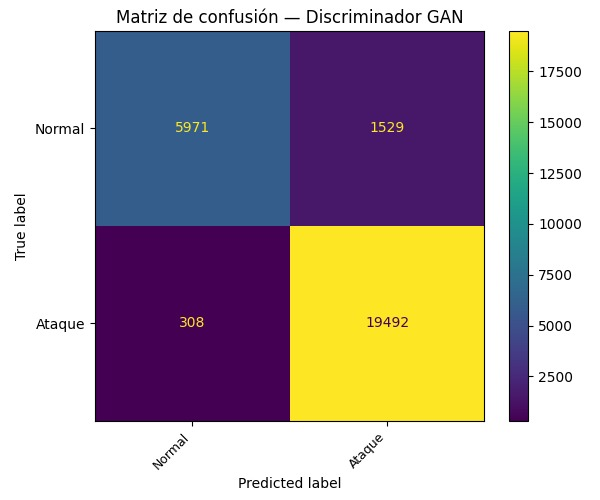
\includegraphics[width=0.70\textwidth]{imagenes/gan_matriz_confusion_test.jpeg}
    \caption{Matriz de confusión do discriminador da GAN sobre o conxunto de test. O modelo detecta correctamente 19\,492 ataques e 5\,971 fluxos normais, con 1\,529 falsos positivos e 308 falsos negativos.}
\end{figure}


A matriz de confusión mostra que a GAN ten unha capacidade moi alta para
detectar ataques, xa que só deixa sen detectar 308 mostras da clase
\texttt{ATTACK}. O principal erro aparece nos falsos positivos: 1\,529 fluxos
normais son clasificados como ataques. Nun contexto de detección de intrusións,
este comportamento é razoábel, xa que é preferíbel xerar algunhas alertas
adicionais antes que deixar pasar tráfico malicioso.


\begin{figure}[H]
    \centering
    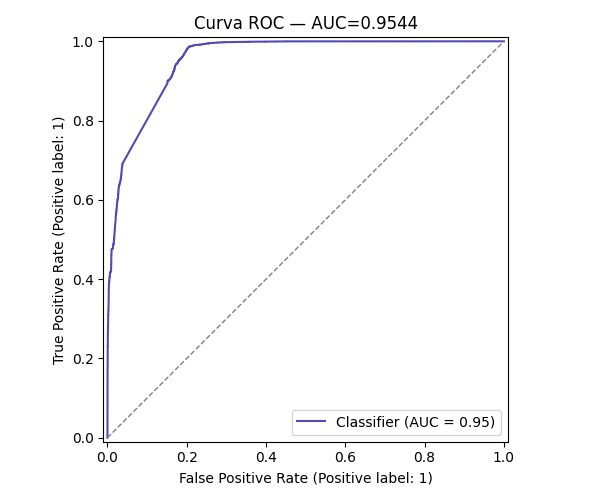
\includegraphics[width=0.70\textwidth]{imagenes/gan_roc_test.jpeg}
    \caption{Curva ROC do discriminador da GAN sobre o conxunto de test. A AUC-ROC acadada é 0,9544.}
\end{figure}


\begin{figure}[H]
    \centering
    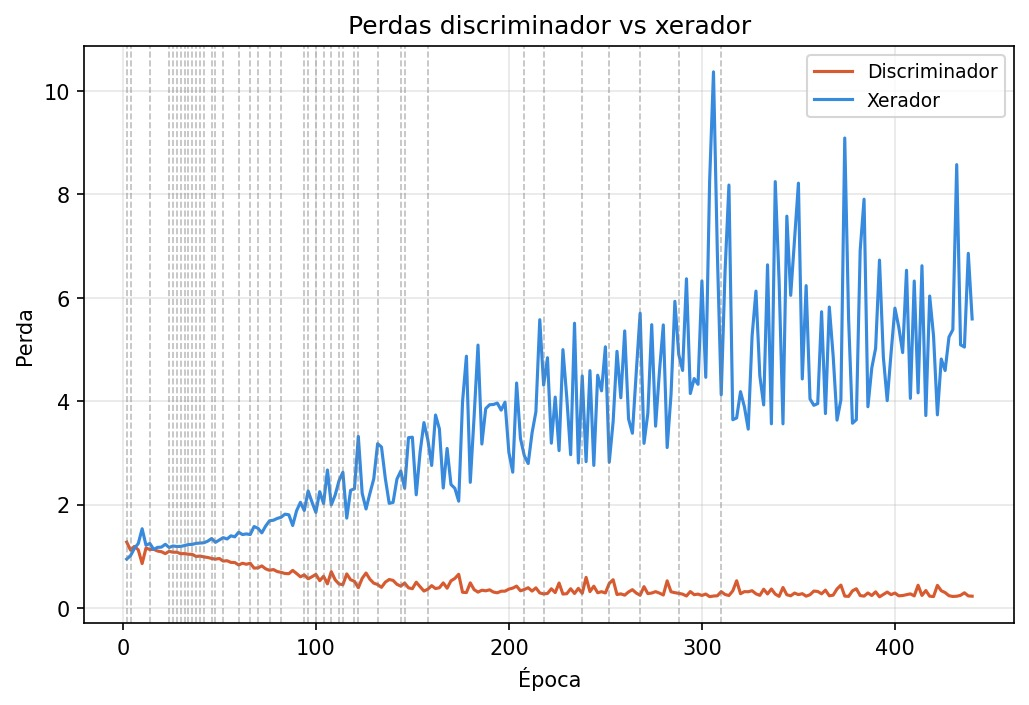
\includegraphics[width=0.92\textwidth]{imagenes/gan_perdas.jpeg}
    \caption{Evolución das perdas do discriminador e do xerador durante o adestramento longo da GAN. Obsérvase que a perda do discriminador diminúe progresivamente mentres que a do xerador tende a aumentar e presenta oscilacións considerábeis, algo habitual no adestramento adversario. As liñas verticais marcan épocas nas que se rexistraron melloras do mellor valor de validación.}
\end{figure}

\begin{figure}[H]
    \centering
    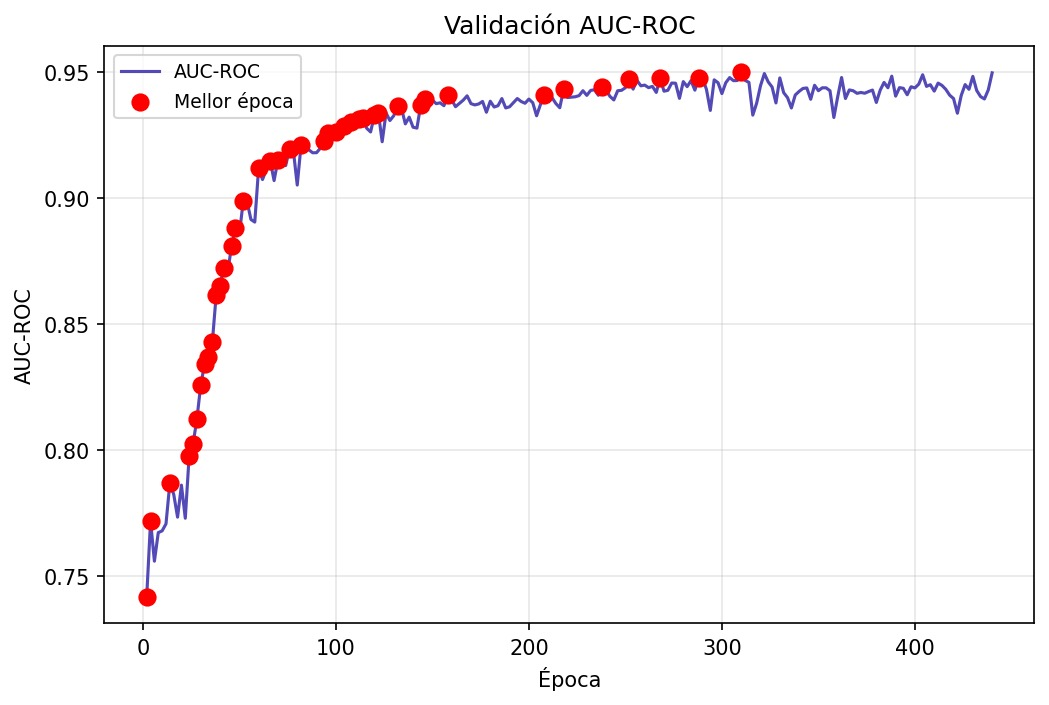
\includegraphics[width=0.85\textwidth]{imagenes/gan_aucroc_validacion.jpeg}
    \caption{Evolución da AUC-ROC de validación ao longo do adestramento da GAN. Os puntos vermellos marcan as épocas nas que se mellorou o mellor valor acadado ata ese momento. Apréciase unha mellora rápida nas primeiras épocas e unha estabilización posterior arredor de 0,94--0,95, cun máximo de 0,9499.}
\end{figure}

\begin{figure}[H]
    \centering
    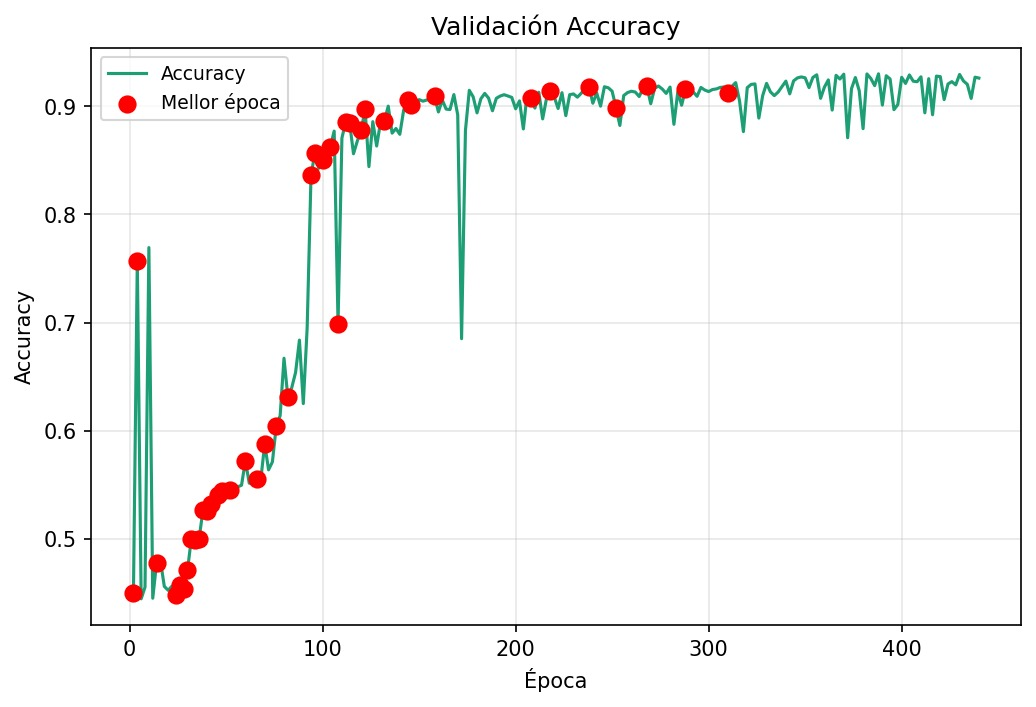
\includegraphics[width=0.85\textwidth]{imagenes/gan_accuracy_validacion.jpeg}
    \caption{Evolución da \emph{accuracy} de validación ao longo do adestramento da GAN. Os puntos vermellos indican as épocas nas que se acadou unha mellora do mellor valor ata o momento. Tras unha fase inicial inestábel, a \emph{accuracy} estabilízase arredor de 0,92--0,93, cun máximo de 0,9300.}
\end{figure}


As tres gráficas de adestramento anteriores amosan o comportamento típico dun
adestramento adversario. Nas primeiras épocas obsérvase unha mellora rápida da AUC-ROC e
da \emph{accuracy} de validación, mentres que posteriormente as curvas se
estabilizan arredor de valores altos. Ao mesmo tempo, as perdas do xerador e
do discriminador presentan oscilacións, o que reflicte a dificultade de
equilibrar ambas redes durante o adestramento.

\subsection{GAN como xerador de datos sintéticos}

Un dos engadidos máis interesantes do traballo foi a implementación dunha
tubaxe de \emph{data augmentation}. Para iso, empregouse o mellor xerador
da GAN para crear novas mostras sintéticas e incorporalas ao conxunto de
adestramento, mantendo sen cambios os conxuntos de validación e test.

O parámetro de proporción permitía controlar cantas mostras reais se mantiñan
no novo conxunto de adestramento e cantas mostras sintéticas se engadían.
Nunha das execucións conservadas xeráronse 127\,400 mostras sintéticas
adicionais, polo que o novo conxunto de adestramento pasou de 127\,400 a
254\,800 mostras.

As mostras xeradas identificáronse como sintéticas no novo conxunto de datos.
Posteriormente, este dataset aumentado empregouse para volver avaliar AdaBoost
no escenario binario, mantendo os mesmos conxuntos de validación e test. Deste
xeito puido comprobarse se a augmentación con mostras xeradas pola GAN melloraba
ou non o rendemento do modelo base.

\section{AdaBoost}

AdaBoost foi o modelo base escollido para a práctica. Trátase dun modelo
supervisado sinxelo, rápido de adestrar e axeitado para datos tabulares, polo
que serve como referencia para comparar fronte á GAN.

Realizouse unha primeira procura mediante \texttt{GridSearchCV},
tanto no caso binario como no multiclase. Esta proba permitiu comprobar que
AdaBoost funcionaba correctamente sobre o dataset preprocesado e obter unha
primeira estimación do rango de hiperparámetros útil.

Na versión final empregouse optimización bayesiana para automatizar
a procura de hiperparámetros \cite{bayopt,Garrido_Merch_n_2020}. O espazo de busca incluíu
\texttt{n\_estimators} entre 15 e 500 e \texttt{learning\_rate} entre 0.0001
e 2. A execución final realizouse con 15 puntos aleatorios iniciais e 40
iteracións adicionais de optimización. A función obxectivo foi o F1 micro en
validación.

AdaBoost avaliouse en dous escenarios diferentes. No primeiro empregáronse
as etiquetas binarias, distinguindo entre \texttt{BENIGN} e \texttt{ATTACK}.
No segundo mantivéronse as etiquetas multiclase orixinais do dataset. Deste
xeito puido estudarse o comportamento do mesmo modelo tanto nun problema
binario como nun problema de clasificación máis detallado.

\subsection{Clasificación binaria}

No escenario binario, AdaBoost obtivo un resultado sólido sobre o conxunto de
test, cunha \emph{accuracy} de 0,9144 e un F1 micro de 0,9144. O modelo
amosou un \emph{recall} moi alto para a clase \texttt{ATTACK}, de 0,98,
sacrificando parte do \emph{recall} da clase \texttt{BENIGN}, que quedou en
0,73. Nun contexto de ciberseguridade, esta compensación é razoábel, xa que
adoita ser preferíbel asumir máis falsos positivos antes que deixar pasar
tráfico malicioso.

O reparto do problema binario no dataset final foi o seguinte:
35\,000 mostras \texttt{BENIGN} e 92\,400 \texttt{ATTACK} no adestramento,
e 7\,500 / 19\,800 tanto en validación como en test.

\begin{table}[H]
\centering
\small
\resizebox{\textwidth}{!}{
\begin{tabular}{lccccccc}
\toprule
\textbf{Modelo} & \textbf{Accuracy} & \textbf{Precision micro} & \textbf{Recall micro} & \textbf{F1 micro} & \textbf{F1 macro} & \textbf{F1 weighted} & \textbf{AUC-ROC} \\
\midrule
AdaBoost binario & 0,9144 & 0,9144 & 0,9144 & 0,9144 & 0,8837 & 0,9106 & 0,9474 \\
\bottomrule
\end{tabular}
}
\caption{Resultados binarios de AdaBoost no conxunto de test}
\end{table}

\begin{figure}[H]
    \centering
    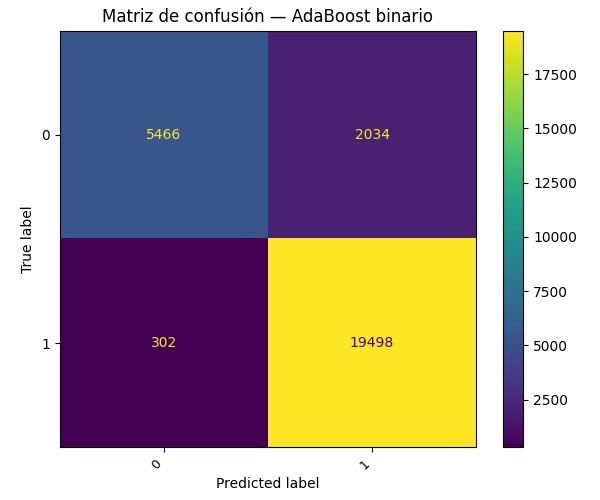
\includegraphics[width=0.65\textwidth]{imagenes/adaboost_matriz_binaria.jpeg}
    \caption{Matriz de confusión de AdaBoost no escenario binario. O modelo clasifica correctamente 5\,466 mostras benignas e 19\,498 ataques, con 2\,034 falsos positivos e 302 falsos negativos.}
\end{figure}

A matriz de confusión de AdaBoost amosa un comportamento semellante ao da GAN:
o modelo detecta case todos os ataques, con só 302 falsos negativos. Porén,
confunde unha parte maior do tráfico benigno, xerando 2\,034 falsos positivos.
Isto explica que o \emph{recall} da clase \texttt{ATTACK} sexa moi alto,
mentres que o \emph{recall} da clase \texttt{BENIGN} queda máis penalizado.

\begin{figure}[H]
    \centering
    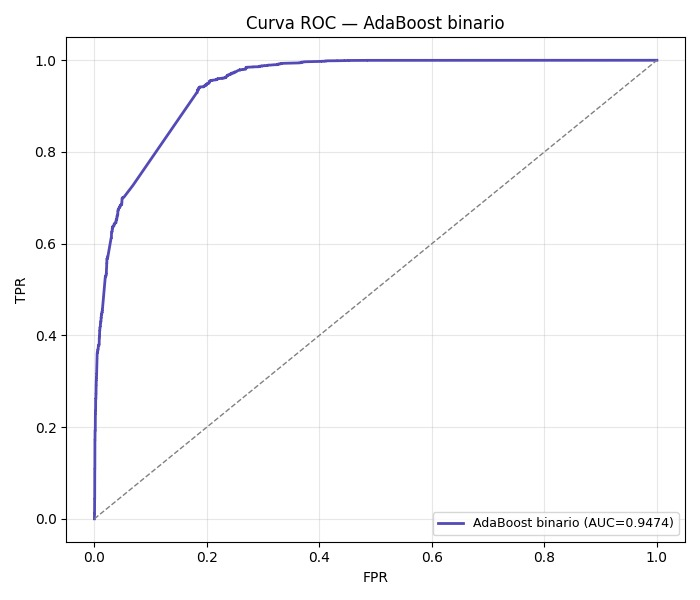
\includegraphics[width=0.70\textwidth]{imagenes/adaboost_roc_binario.jpeg}
    \caption{Curva ROC de AdaBoost no escenario binario. A AUC-ROC acadada sobre o conxunto de test é 0,9474.}
\end{figure}

As figuras seguintes recollen a evolución da busca bayesiana no caso binario.
Obsérvase a converxencia do máximo acumulado e a localización das mellores
combinacións no espazo de parámetros.

\begin{figure}[H]
    \centering
    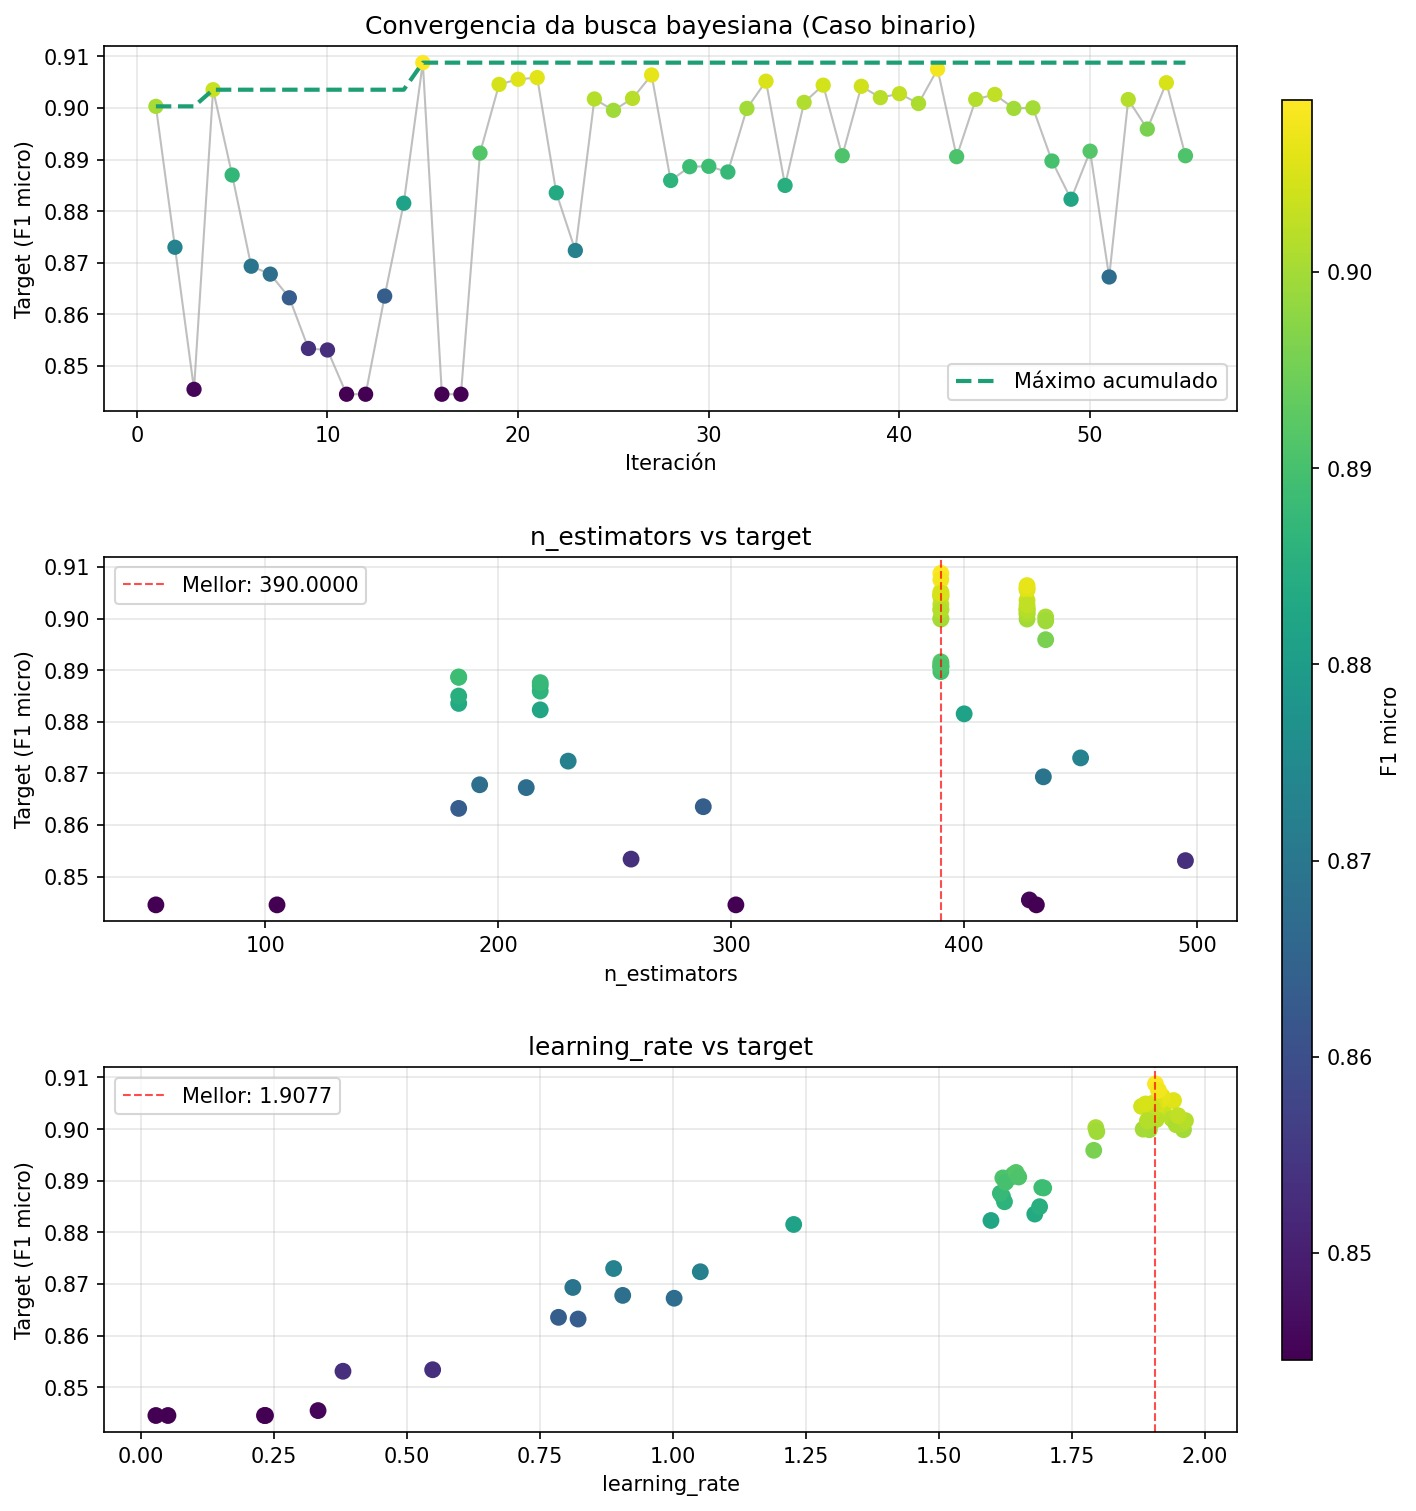
\includegraphics[width=0.93\textwidth]{imagenes/adaboost_bayes_binario_convergencia.jpeg}
    \caption{Converxencia da busca bayesiana de AdaBoost no caso binario. O mellor valor aproxímase a F1 micro $\approx 0{,}909$, cun \texttt{n\_estimators} próximo a 390 e \texttt{learning\_rate} arredor de 1,908.}
\end{figure}

\begin{figure}[H]
    \centering
    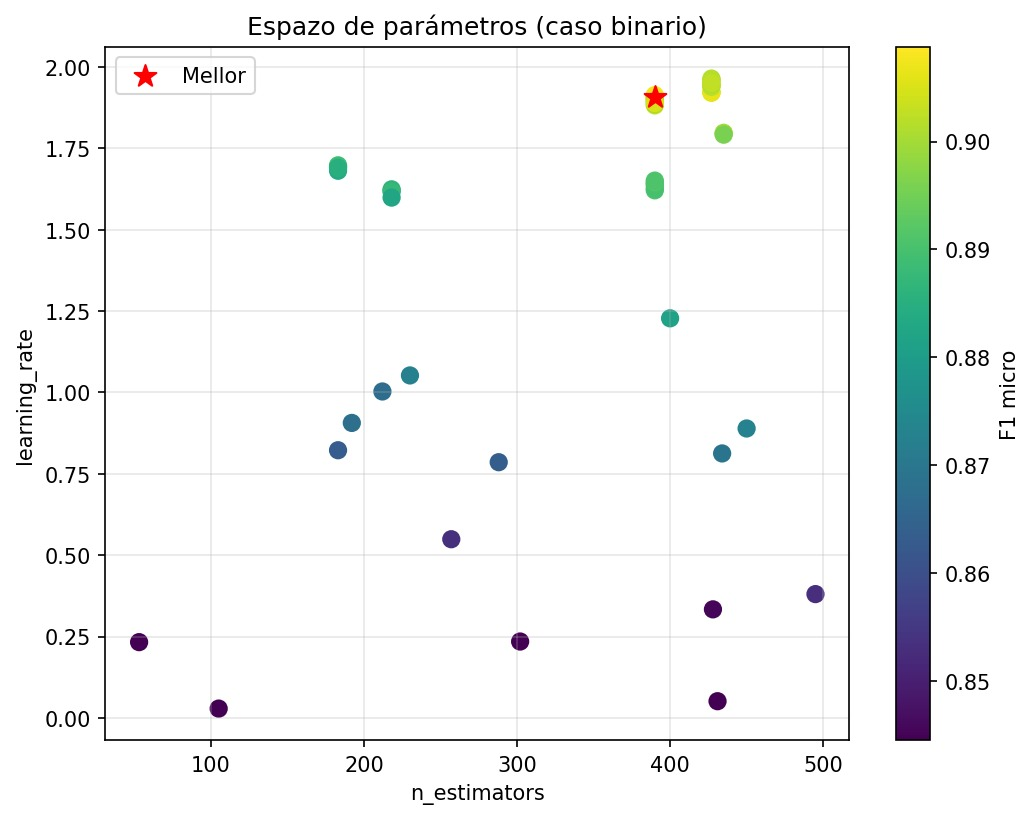
\includegraphics[width=0.70\textwidth]{imagenes/adaboost_bayes_binario_espazo.jpeg}
    \caption{Espazo de parámetros explorado para AdaBoost no caso binario. A concentración de puntos de maior calidade aparece na zona de \texttt{learning\_rate} alto e número de estimadores medio-alto.}
\end{figure}


\subsection{Clasificación multiclase}

Tamén se estudou unha extensión multiclase. Neste escenario mantéñense as
etiquetas orixinais do dataset, polo que o problema é máis difícil ca no caso
binario: ademais de distinguir tráfico benigno fronte a ataque, o modelo debe
identificar o tipo concreto de tráfico ou ataque.

Na avaliación multiclase, AdaBoost acadou unha \emph{accuracy} de 0,65,
cun \emph{macro F1} de 0,47 e un \emph{weighted F1} de 0,62. As clases
maioritarias e algunhas firmas específicas como \texttt{SSH-Patator},
\texttt{PortScan} ou \texttt{DDoS} tiveron un comportamento aceptábel, pero
as clases moi raras ou máis difíciles, como \texttt{Heartbleed},
\texttt{Web Attack - Brute Force}, \texttt{Web Attack - Sql Injection} e
\texttt{Web Attack - XSS}, seguiron moi penalizadas.

\begin{table}[H]
\centering
\small
\caption{Resumo das métricas multiclase de AdaBoost}
\begin{tabular}{lcccc}
\toprule
\textbf{Modelo} & \textbf{Accuracy} & \textbf{Macro precision} & \textbf{Macro recall} & \textbf{Macro F1} \\
\midrule
AdaBoost multiclase & 0,65 & 0,58 & 0,45 & 0,47 \\
\bottomrule
\end{tabular}
\end{table}

\begin{table}[H]
\centering
\small
\caption{Métricas ponderadas da avaliación multiclase}
\begin{tabular}{lccc}
\toprule
\textbf{Modelo} & \textbf{Weighted precision} & \textbf{Weighted recall} & \textbf{Weighted F1} \\
\midrule
AdaBoost multiclase & 0,66 & 0,65 & 0,62 \\
\bottomrule
\end{tabular}
\end{table}

\begin{table}[H]
\centering
\small
\caption{AUC-ROC one-vs-rest de AdaBoost no escenario multiclase}
\begin{tabular}{lc}
\toprule
\textbf{Clase} & \textbf{AUC-ROC} \\
\midrule
\texttt{BENIGN} & 0,7956 \\
\texttt{Bot} & 1,0000 \\
\texttt{DDoS} & 0,9506 \\
\texttt{DoS GoldenEye} & 0,9310 \\
\texttt{DoS Hulk} & 0,8956 \\
\texttt{DoS Slowhttptest} & 0,8387 \\
\texttt{DoS slowloris} & 0,9199 \\
\texttt{FTP-Patator} & 0,9998 \\
\texttt{Heartbleed} & 0,9977 \\
\texttt{Infiltration} & 0,9205 \\
\texttt{PortScan} & 0,8888 \\
\texttt{SSH-Patator} & 0,9994 \\
\texttt{Web Attack - Brute Force} & 0,9073 \\
\texttt{Web Attack - Sql Injection} & 0,8601 \\
\texttt{Web Attack - XSS} & 0,9179 \\
\bottomrule
\end{tabular}
\end{table}

\begin{figure}[H]
    \centering
    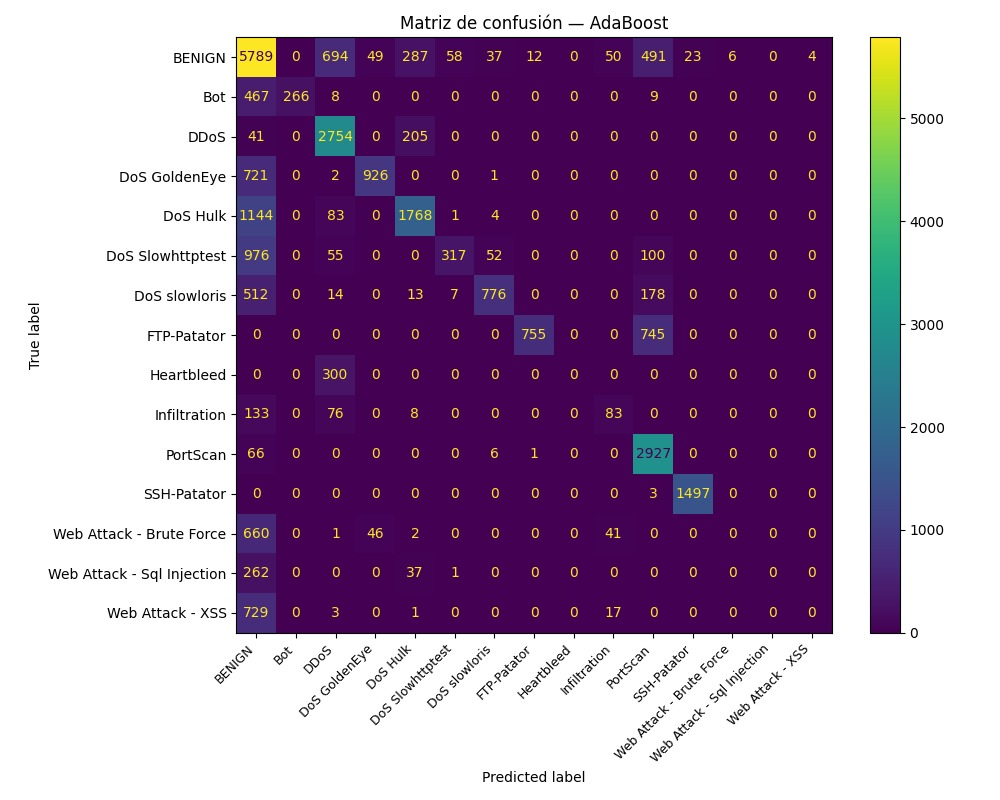
\includegraphics[width=0.95\textwidth]{imagenes/adaboost_matriz_multiclase.jpeg}
    \caption{Matriz de confusión de AdaBoost no escenario multiclase. Obsérvase un bo comportamento en clases como \texttt{DDoS}, \texttt{PortScan} e \texttt{SSH-Patator}, mentres que varias clases minoritarias quedan confundidas con \texttt{BENIGN} ou con outras clases maioritarias.}
\end{figure}

No caso multiclase obsérvase unha dificultade maior. O modelo identifica ben
algunhas clases con patróns máis definidos, como \texttt{SSH-Patator},
\texttt{DDoS} ou \texttt{PortScan}, pero varias clases minoritarias aparecen
mal clasificadas ou directamente absorbidas por clases máis frecuentes. Isto
é coherente coas métricas macro, que son máis baixas ca as ponderadas, e indica
que o rendemento global está influído polas clases maioritarias.

\begin{figure}[H]
    \centering
    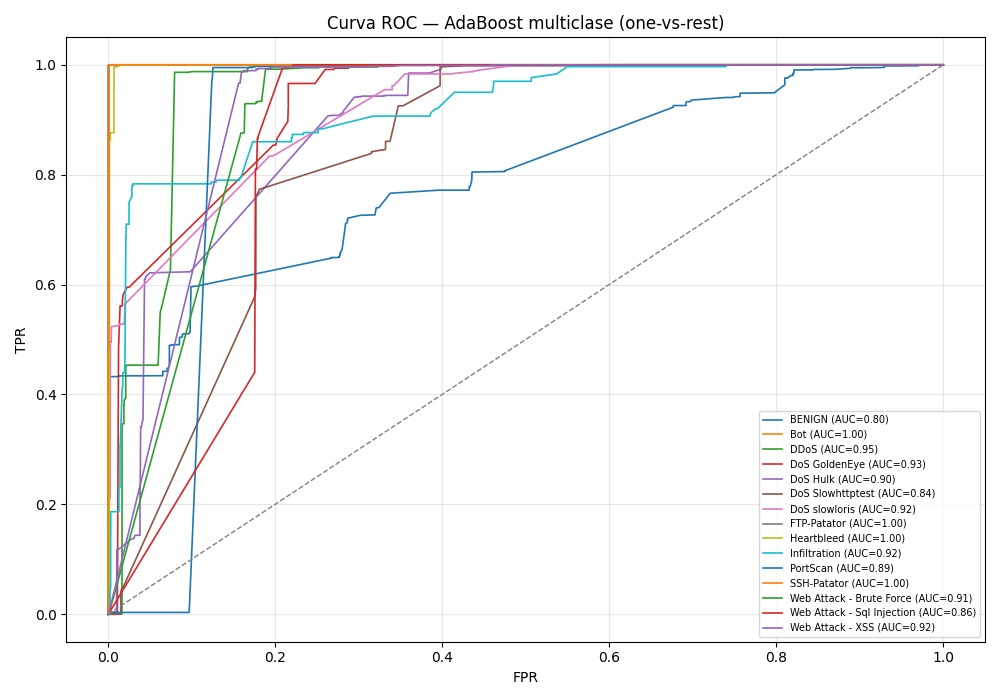
\includegraphics[width=0.95\textwidth]{imagenes/adaboost_roc_multiclase.jpeg}
    \caption{Curvas ROC one-vs-rest de AdaBoost no escenario multiclase. A maioría das clases presentan unha AUC elevada, aínda que a clase \texttt{BENIGN} obtén un valor menor, con AUC-ROC de 0,7956.}
\end{figure}

As figuras seguintes recollen a evolución da busca bayesiana no caso
multiclase.

\begin{figure}[H]
    \centering
    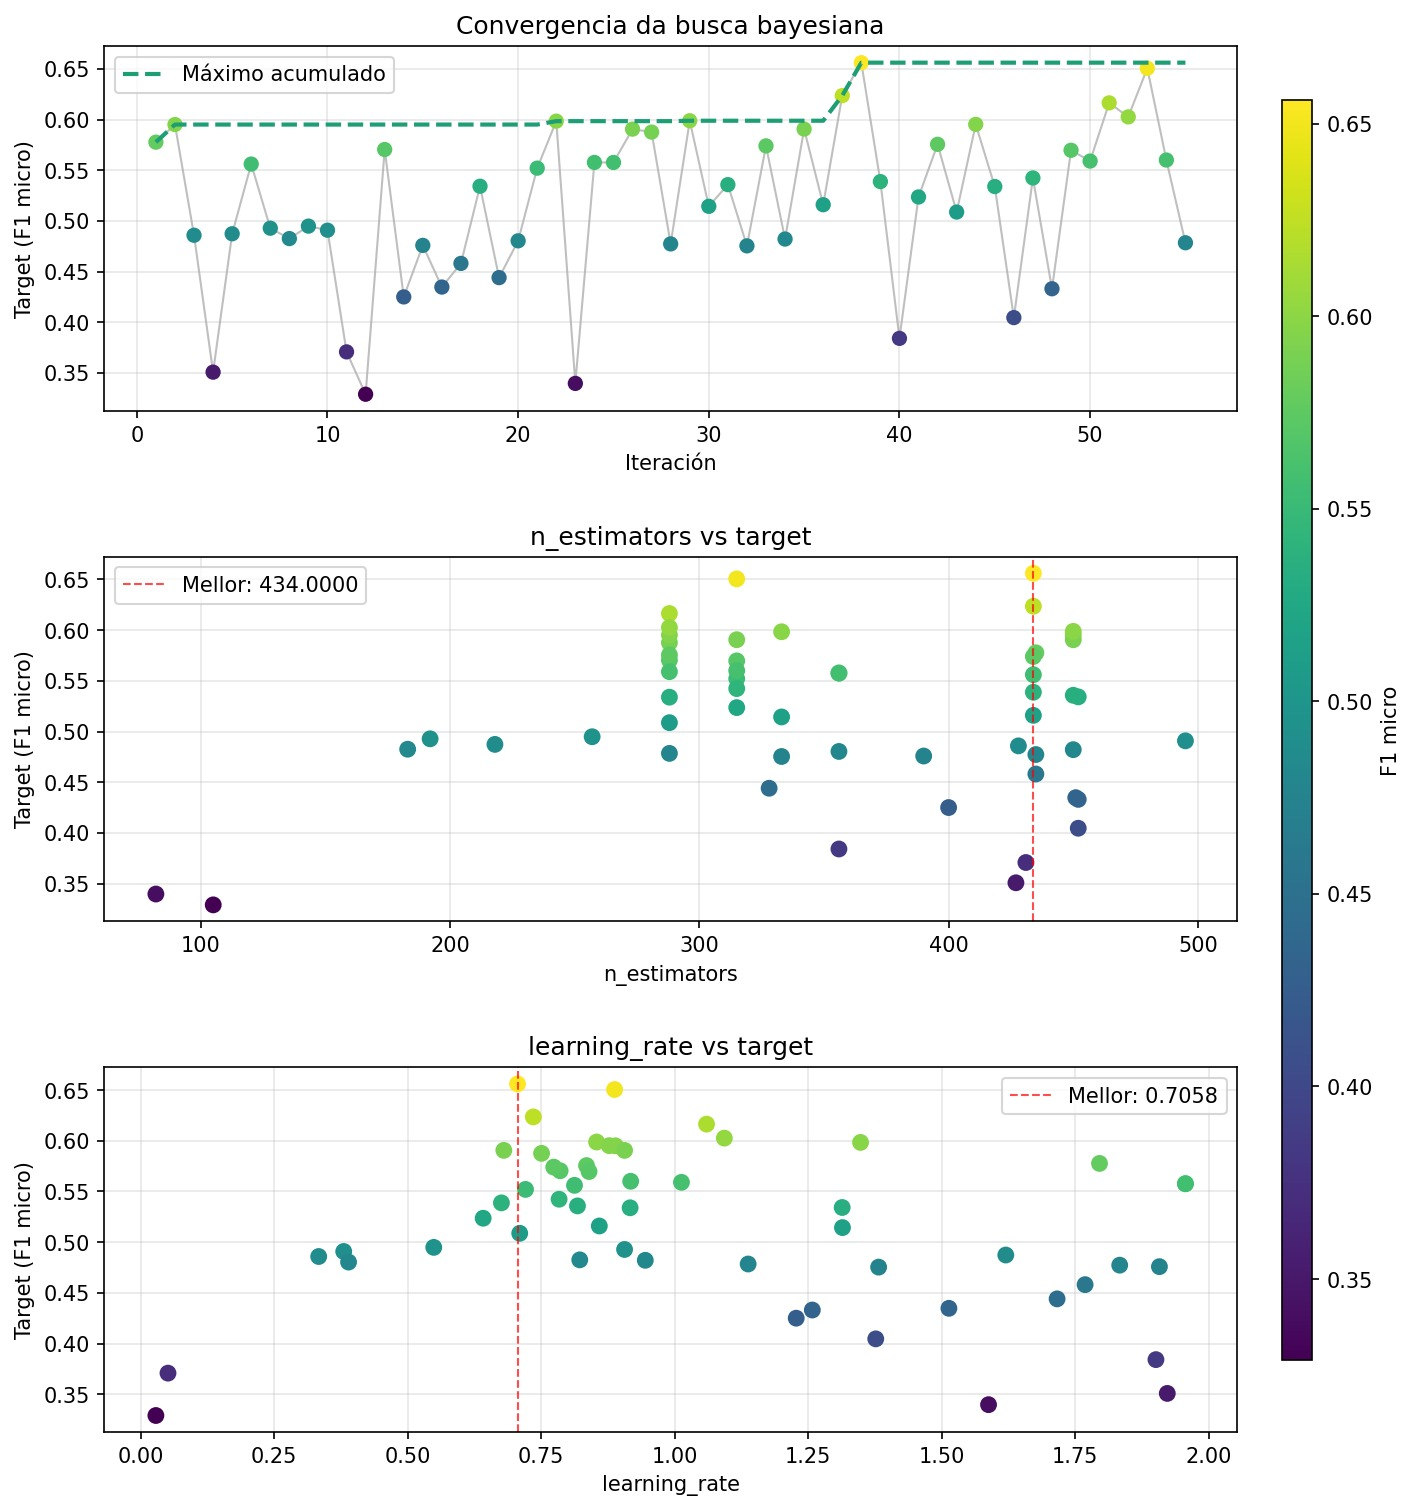
\includegraphics[width=0.93\textwidth]{imagenes/adaboost_bayes_multiclase_convergencia.jpeg}
    \caption{Converxencia da busca bayesiana de AdaBoost no caso multiclase. Obsérvase un mellor valor arredor de F1 micro $\approx 0{,}656$, con \texttt{n\_estimators} próximo a 434 e \texttt{learning\_rate} arredor de 0,706.}
\end{figure}

\begin{figure}[H]
    \centering
    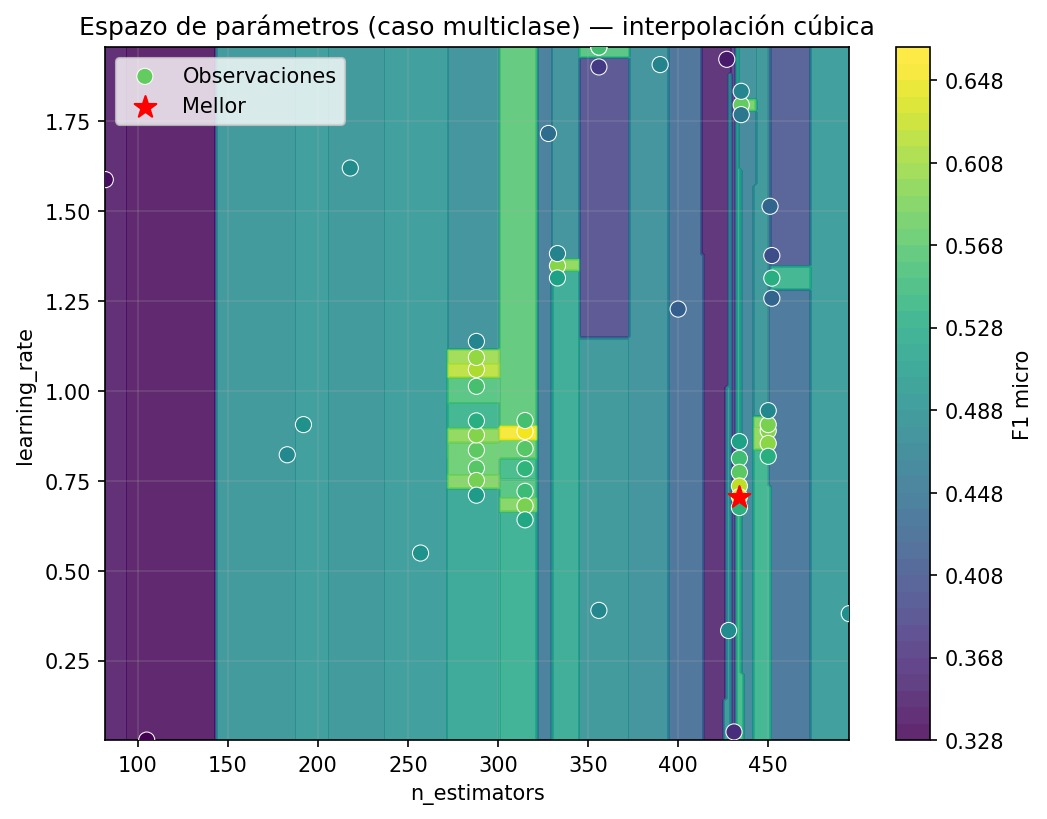
\includegraphics[width=0.70\textwidth]{imagenes/adaboost_bayes_multiclase_espazo.jpeg}
    \caption{Espazo de parámetros explorado para AdaBoost no caso multiclase. A estrela sinala a mellor combinación atopada pola optimización bayesiana.}
\end{figure}


\subsection{Dataset aumentado}

A continuación de empregar a GAN como xerador, avaliouse tamén o uso de
mostras sintéticas como técnica de \emph{data augmentation}. O obxectivo era
comprobar se engadir datos xerados pola GAN ao conxunto de adestramento podía
mellorar o rendemento de AdaBoost no escenario binario.

Nunha das execucións conservadas xeráronse 127\,400 mostras sintéticas
adicionais, polo que o conxunto de adestramento pasou de 127\,400 a
254\,800 mostras. Mantivéronse os mesmos conxuntos de validación e test, de
maneira que a comparación co AdaBoost adestrado co dataset orixinal fose
directa.

\begin{table}[H]
\centering
\small
\resizebox{\textwidth}{!}{
\begin{tabular}{lcccccc}
\toprule
\textbf{Modelo} & \textbf{Accuracy} & \textbf{Precision micro} & \textbf{Recall micro} & \textbf{F1 micro} & \textbf{F1 macro} & \textbf{F1 weighted} \\
\midrule
AdaBoost con dataset aumentado & 0,9112 & 0,9112 & 0,9112 & 0,9112 & 0,8806 & 0,9078 \\
\bottomrule
\end{tabular}
}
\caption{Resultados binarios de AdaBoost empregando o dataset aumentado pola GAN}
\end{table}

O resultado obtido foi moi semellante ao do AdaBoost adestrado co dataset
orixinal. Co dataset orixinal obtívose unha \emph{accuracy} de 0,9144 e un
F1 weighted de 0,9106, mentres que co dataset aumentado a \emph{accuracy}
foi de 0,9112 e o F1 weighted de 0,9078. Polo tanto, a augmentación con datos
sintéticos non produciu unha mellora apreciábel neste experimento.

\begin{figure}[H]
    \centering
    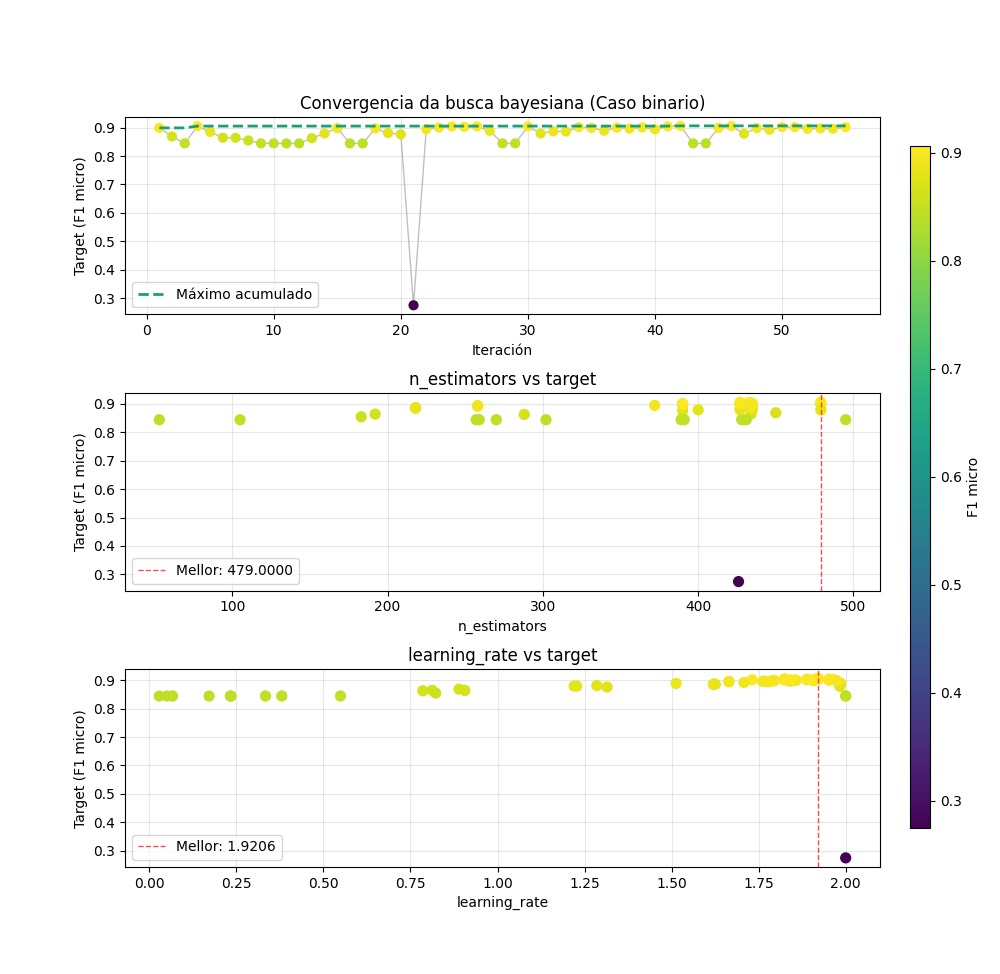
\includegraphics[width=0.90\textwidth]{imagenes/adaboost_aug_binario_convergencia.jpeg}
    \caption{Converxencia da busca bayesiana de AdaBoost no caso binario empregando o dataset aumentado. O mellor valor mantense arredor de F1 micro $\approx 0{,}91$, moi próximo ao obtido co dataset orixinal.}
\end{figure}

\begin{figure}[H]
    \centering
    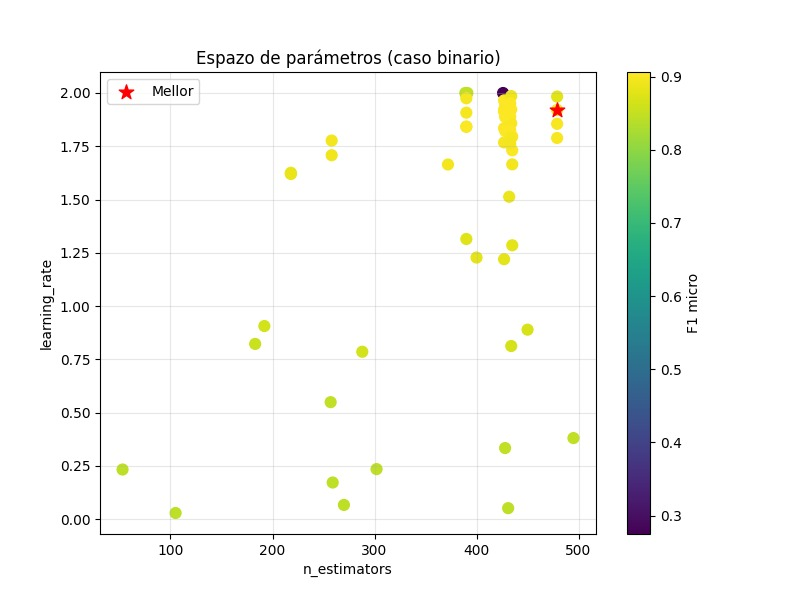
\includegraphics[width=0.70\textwidth]{imagenes/adaboost_aug_binario_espazo.jpeg}
    \caption{Espazo de parámetros explorado para AdaBoost no caso binario co dataset aumentado. A mellor configuración aparece nunha zona de número alto de estimadores e \emph{learning rate} elevado, semellante ao observado no dataset orixinal.}
\end{figure}

A explicación máis probábel é que o xerador aínda non reproduce con suficiente
fidelidade a distribución real dos datos. No adestramento dunha GAN, primeiro
é habitual que o discriminador aprenda a separar mellor as mostras reais das
xeradas; só despois, cando esa sinal de erro é útil, o xerador comeza a
mellorar progresivamente. Aínda que o discriminador acadou bos resultados como
clasificador, iso non garante que as mostras sintéticas xeradas teñan a mesma
calidade estatística ca os datos reais. Por este motivo, ao engadilas ao
adestramento de AdaBoost, o efecto final foi practicamente neutro.

\section{Comparativa}

A comparación entre ambos modelos xa pode facerse con métricas de test no
escenario binario. AdaBoost ofrece un modelo base rápido e estábel, mentres
que a GAN require máis axuste e un adestramento máis longo, pero acada mellores
métricas finais no test binario conservado.

En primeiro lugar, AdaBoost foi o mellor modelo base do traballo. A súa principal vantaxe é a eficiencia: adéstrase rápido, é doado de 
optimizar e ofrece un rendemento moi competitivo no problema binario. Ademais, a interpretación das súas métricas é directa e permite construír 
unha memoria máis limpa e reproducíbel.

En segundo lugar, a GAN xustifica a súa presenza como modelo complexo precisamente porque introduce dificultades reais de adestramento. 
As probas curtas demostraron que a converxencia non chega en poucas épocas; o \emph{dropout}, a configuración do adestramento e o número de iteracións inflúen 
moito máis do esperado. Por outra banda, cando se lle dedica tempo dabondo, o discriminador consegue
métricas altas en validación, chegando a unha AUC-ROC próxima a 0,95, e o
xerador abre a porta á creación de novos datasets.

\begin{table}[H]
\centering
\small
\resizebox{\textwidth}{!}{
\begin{tabular}{lccccc}
\toprule
\textbf{Modelo} & \textbf{Accuracy} & \textbf{Precision ATTACK} & \textbf{Recall ATTACK} & \textbf{F1 ATTACK} & \textbf{AUC-ROC} \\
\midrule
AdaBoost & 0,9144 & 0,91 & 0,98 & 0,94 & 0,9474 \\
AdaBoost con dataset aumentado & 0,9112 & 0,91 & 0,98 & 0,94 & -- \\
GAN & 0,9327 & 0,9273 & 0,9844 & 0,9550 & 0,9544 \\
\bottomrule
\end{tabular}
}
\caption{Comparativa cuantitativa no escenario binario sobre test}
\end{table}


O AdaBoost adestrado co dataset aumentado obtivo métricas moi próximas ás do
AdaBoost adestrado só cos datos reais, pero sen melloralas. Isto indica que,
nesta configuración, as mostras sintéticas xeradas pola GAN non achegaron
información adicional suficiente para mellorar a fronteira de decisión do
modelo base.

En resumo, se se valora a simplicidade, a velocidade e a estabilidade do
adestramento, AdaBoost é a opción máis práctica. Se se atende ás métricas
obtidas no test binario conservado, a GAN acada mellores resultados, aínda
que cun custo de axuste e adestramento maior. Ademais, a GAN achega unha
utilidade adicional ao permitir xerar mostras sintéticas.

\section{Conclusións}

O traballo permitiu completar o obxectivo principal da práctica: adestrar e
comparar dous modelos diferentes sobre CIC-IDS2017, partindo do preprocesado
realizado na primeira entrega e analizando os resultados obtidos.

AdaBoost consolidouse como unha solución base moi forte no escenario binario.
Coa configuración axeitada ofreceu métricas altas, un tempo de execución
reducido e unha interpretación clara dos resultados. Por iso pode considerarse
o modelo máis práctico e estábel do traballo, aínda que a GAN acadase mellores
métricas no test binario conservado.

A GAN foi máis esixente. As probas iniciais non chegaron a converxer, pero os adestramentos longos demostraron que o discriminador podía acadar resultados
competitivos tanto en validación como no conxunto de test. Ademais, o feito de reutilizar o xerador para producir novas mostras permitiu
avaliar a GAN como ferramenta de augmentación de datos, aínda que nesta
execución concreta non se obtivo unha mellora apreciábel en AdaBoost.

A conclusión global é que AdaBoost ofrece a mellor relación entre
simplicidade, estabilidade e custo de adestramento, mentres que a GAN acada
mellores métricas no test binario conservado e introduce flexibilidade
adicional ao permitir a xeración de mostras sintéticas. Esa combinación fai
que a comparativa entre ambos modelos sexa rica e xustificábel.

\section{Traballo Futuro}

A partir dos resultados obtidos, as principais liñas de mellora serían as
seguintes:

\begin{itemize}[leftmargin=1.5em]

    \item Explorar variantes máis específicas da GAN, como GANs condicionais
    ou unha GAN independente por clase, no caso de querer abordar o problema
    multiclase con maior profundidade. Ademais, esa GAN condicional, unha vez adestrada,
    podería ser de utilidade (independentemente do seu rendemento en clasificación multiclase)
    como xerador de mostras sintéticas para adestrar un AdaBoost multiclase mellorado.

    \item Implementar unha búsqueda máis profunda sobre o espazo de parámetros para o caso multiclase de AdaBoost,
          tanto de puntos iniciais como de profundidade da búsqueda bayesiana, esperando mellorar o seu rendemento, 
          sobre todo nas clases minoritarias.



\end{itemize}

\newpage

\bibliographystyle{IEEEtran}
\bibliography{licencias}

\end{document}
